The chapter addresses the problem of optimally controlling an industrial micro-grid featuring a large share of renewable energy and a high volatility of electricity prices. We consider a micro-grid as a localized group of energy sources, loads and storage components that can operate in two distinct modes: grid-connected mode and isolated mode. In grid-connected mode, the micro-grid system has the possibility to buy/sell energy from/to the macro-grid in order to meet the load demand. The challenge in connected mode is to reduce the total energy cost. In isolated mode, the micro-grid can function autonomously in the sense that enough energy can be generated in the grid to supply the loads. In this case the challenge is to meet the load demand and to balance the power flow between the components of the grid. In our setting, the grid is executed in mixed mode. In other words, the industrial micro-grid, we are considering, can switch from one mode to another.

\subsection{System Model}
\label{subsec:31}

% For figures use
%
\begin{figure}[b]
%\sidecaption
% Use the relevant command for your figure-insertion program
% to insert the figure file.
% For example, with the graphicx style use
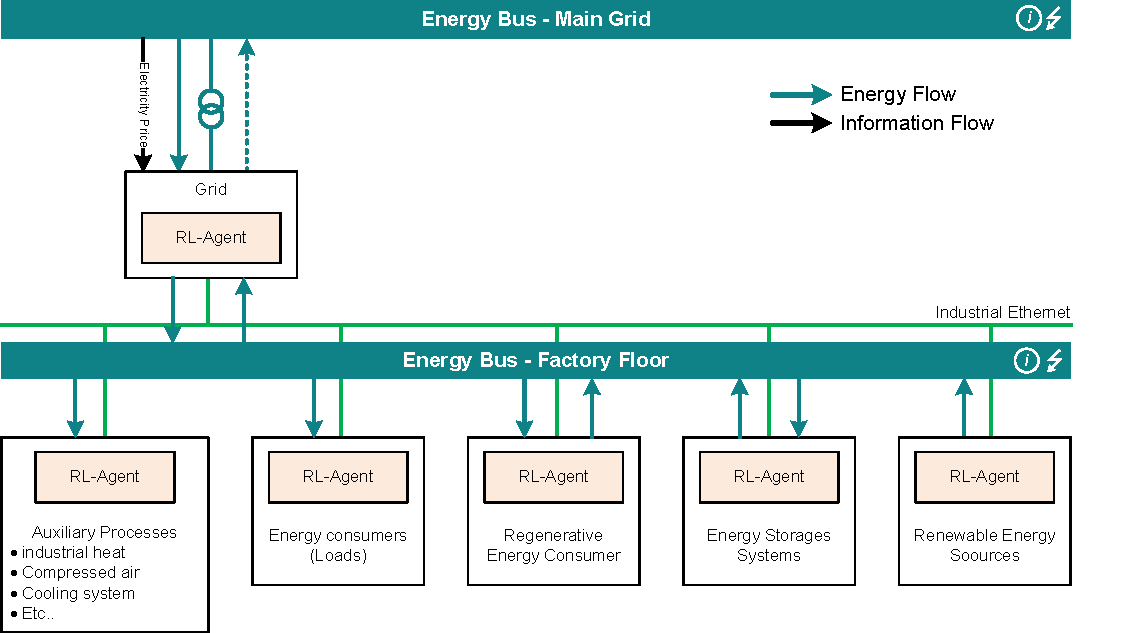
\includegraphics[scale=.65]{images/System_Model}
%
% If no graphics program available, insert a blank space i.e. use
%\picplace{5cm}{2cm} % Give the correct figure height and width in cm
%
\caption{System Overview. Every grid-component is controlled by a reinforcement learning agent.}
\label{fig:system_model}       % Give a unique label
\end{figure}

As illustrated in Fig.\ref{fig:system_model}, the micro-grid system consists of the following components: renewable energy sources such as PV-Arrays, electricity loads representing production machines, regenerative energy consumers, energy storages systems such as batteries and auxiliary process loads for air compressors and cooling systems. The components share the same energy bus, enabling a transfer of electrical energy between the components. The proposed system model is equally applicable to ac and dc micro-grids and a simple formal description of the components can be described as follow:
\begin{itemize}
\item{\textit{\textbf{ Renewable energy sources}} are renewable energy generators such as PV-Arrays or wind turbines. The power generated depends on environmental and weather factors such as solar radiation profile and wind speed. It is therefore not predictable. Energy generators are characterized by two operating states: $on$ and $off$. The generators are considered to be in the $off$-state when the electrical power generated by the energy sources is negligible for example because of weather conditions such as cloudy weather or nighttime. We assume that if the generators are not in $off$ state, then the power generated is constant and equal to the maximum electricity power that can be produced by the source. Therefore
%
\begin{equation}
 P_G = 
 \begin{cases}
      0 & \text{if}\ state=off \\
      P_Gmax & \text{otherwise}
    \end{cases} \;
\end{equation}
%
 } 
\item{\textit{\textbf{Energy storage systems}}. In order to take full advantage of renewable energy sources, it is vital to have energy storage systems capable of handling variations in energy production. In our environment, we consider batteries or super-capacitor systems that consume a constant energy when charging and produce a constant energy when discharging. In addition, the operation of energy storage systems has to be carefully designed and controlled to protect them from damages that are: overcharging and overdischarging. Therefore, each storage system is also characterized by a maximum and minimum state-of-charge (SoC). The energy storage systems have three required states: $charging$, $discharging$ and $idle$. The electrical power consumed or released by the component highly depends on the current operational state and the component\rq{s} state-of-charges.}
 
 \item{\textit{\textbf{Energy loads}} represent production machines that consume energy in order to execute a production task. A production machine can have different operation states: $powered off$, $executing$, $stand by$, etc… Depending on the production task and the operation state, a production machine can follow a predefined or a characteristic load profile. For a fixed set of production tasks, the load profile of a machine can be measured and approximated. In our setting, we consider 3 basic load profile as illustrated in Fig. \ref{fig:load_profile}. Any machine\rq{s} load profile can be seen as a linear combination of this basic load profiles. In isolated mode, the micro-grid cannot guarantee continuous power supply to the load because it is often influenced by the unpredictable power generation. When the generated power is not able to drive the loads, the noncritical loads must shut down.}
 
 % For figures use
%
\begin{figure}[h!]
%\sidecaption
% Use the relevant command for your figure-insertion program
% to insert the figure file.
% For example, with the graphicx style use
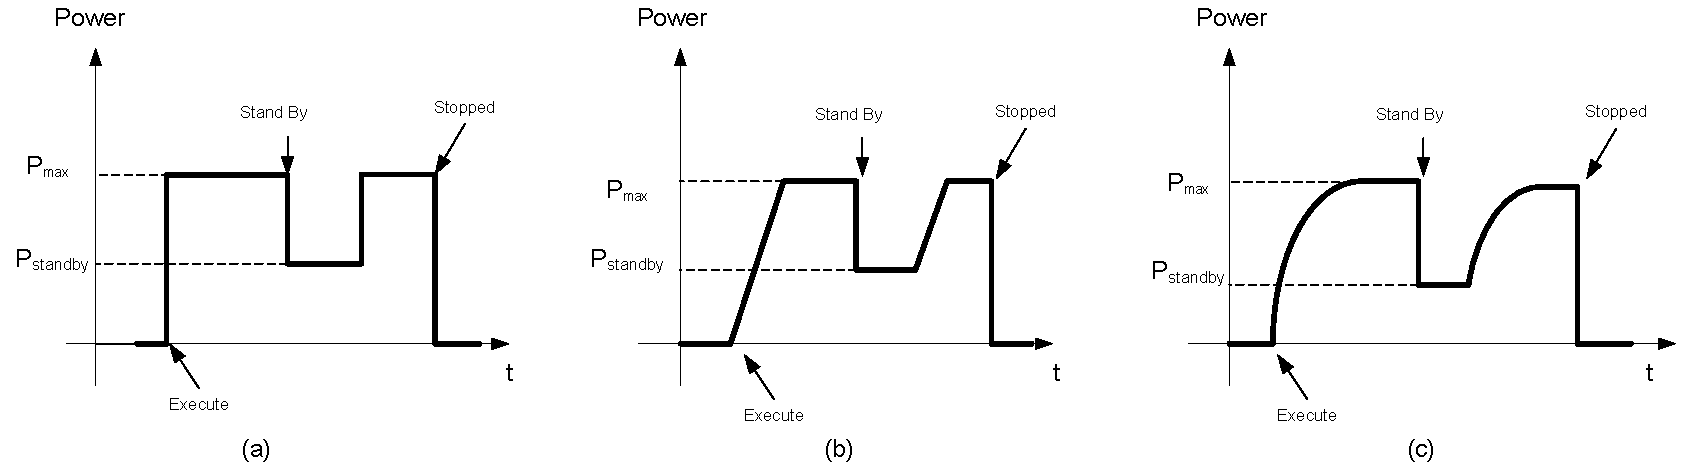
\includegraphics[scale=.40]{images/load_profile}
%
% If no graphics program available, insert a blank space i.e. use
%\picplace{5cm}{2cm} % Give the correct figure height and width in cm
%
\caption{Basic load profiles of the energy loads. In $execute$-state,  the electrical power consumed $P_i$ can be constant and equal to $P_{max}$ (a), increase linearly (b) or exponentially (c) to $P_{max}$.}
\label{fig:load_profile}       % Give a unique label
\end{figure}

 
\item{\textit{\textbf{Regenerative energy consumers}} are energy consumers with the exception that these consumers can recuperate energy for a small period of time (less than a minute). In this case we consider the load to be constant and negative. Fig. \ref{fig:recuperative_load_profile} shows a typical load profile.}

 % For figures use
%
\begin{figure}[h!]
\sidecaption
% Use the relevant command for your figure-insertion program
% to insert the figure file.
% For example, with the graphicx style use
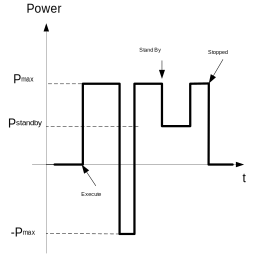
\includegraphics[scale=.40]{images/Recuperative_Energy_Load_Profile}
%
% If no graphics program available, insert a blank space i.e. use
%\picplace{5cm}{2cm} % Give the correct figure height and width in cm
%
\caption{Basic load profiles of regenerative energy consumers. In $execute$-state,  the electrical power consumed $P_i$ can be negative for a short period of time.}
\label{fig:recuperative_load_profile}       % Give a unique label
\end{figure}


\item{\textit{\textbf{Auxiliary processes}} are energy consumer processes in the factory floor that do not execute a manufacturing task directly, but are required by the production task. These are for example compressors or cooling systems. Auxiliary processes have two required states: $off$ and $on$.}

\item{The \textit{\textbf{grid component}} represents the main grid and is responsible for buying/selling electricity from/to the main grid. It has three state: $buying$, $selling$, $idle$. If the grid agent is in $idle$-state or in $off$-state, the industrial micro-grid can be considered to be executed in isolated mode because there are no interaction with the main grid.}
\end{itemize}

\subsection{Problem Formulation}
The main objective is to minimize the total cost the energy bought from the main grid to achieve a high productivity while considering future energy prices and weather dependent renewable energy generators. Let $\mathrm{M}$ denotes the set of components of the micro-grid (or controllable machine components), such that $M_i \in \mathrm{M}, \forall i \in [0, M-1]$  with $ M \in \mathbb{N}$. We assume that each component $M_i$ can take an energy state $s_{i,t}$ (i.e. “stopped”, “running”, “aborted”, “standby”, etc.) at the time step $t  \in \mathbb{N}$ and the dynamic power consumption $P_i^t$ of $M_i$ solely depends on the current state $s_{i,t}$ of the component and the current time step $t$: $P_i^t=P_i (t, s_{i,t})$. The total energy requested/sold from/to the main grid $E_i^t$ at time interval $\triangle t$ over the complete time horizon $T \in \mathbb{N}$ is therefore the sum of the power consumed/generated of all components during the time horizon. Please notice that $P_i^t$ can also be negative in the case of renewable energy sources or regenerative energy consumers for example.

%
\begin{equation}
E_i =\sum_{t=0}^{T-1}{ P_i^t \cdot \triangle t}, \forall i \in [0, M-1]
\end{equation}
%

 If $\lambda_t^- \in \mathbb{R}$ is the actual energy price and $\lambda_t^\sim \in \mathbb{R}$ the forecasted energy price at a time step $t$, the optimization problem can be formulated for the time horizon $T$ as follow:

%
\begin{equation}
\label{eq:problem}
minimize \sum_{k=0}^{t}{ {\lambda_t^-} \cdot ({ \sum_{i=0}^{M-1}{ P_i (k, s_{i,k}) \cdot \triangle t } })}+  \sum_{l=t+1}^{T-1}{\lambda_t^\sim \cdot ({ \sum_{i=0}^{M-1}{ P_i (l, s_{i,l}) \cdot \triangle t  } }) }
\end{equation}

If $a_l (s_{i,l-1},s_{i,l})$ denotes the action of changing the state of the component $M_i$ at time $l$ from the state $s_(i,l-1)$ to the state $s_(i,l)$, the Eq. \ref{eq:problem} can be rewritten as follow:

\begin{equation}
\label{eq:problem_reformulated}
minimize \sum_{k=0}^{t}{ {\lambda_t^-} \cdot ({ \sum_{i=0}^{M-1}{ P_i (k, s_{i,k}) \cdot \triangle t } })}+  \sum_{l=t+1}^{T-1}{\lambda_t^\sim \cdot ({ \sum_{i=0}^{M-1}{ P_i (l, a_l (s_{i,l-1},s_{i,l})) \cdot \triangle t  } }) }
\end{equation}

Several constraints should be taken into consideration. One of them is the power balance between the energy demand of the micro-grid and the energy supply from the main grid:

\begin{equation}
\label{eq:constraint_energy_balance}	
	\sum_{i=0}^{M-1}{ E_i} \leq E_{max}^\sim,  \forall i \in [0, M-1]
\end{equation}
where $E_i$ denotes the total energy demand of the micro-grid component $M_i$ over the time horizon $T$ and $E_{max}^\sim$ the total available energy from the main grid.

In addition, the total energy consumption of the micro-grid at each time interval $t$ should satisfy the upper and lower bound given by the overall load profile and a tolerance interval. This constraint can be expressed as follows:

\begin{equation}
\label{eq:constraint_load_profile}	
	L_{target}^\sim - \triangle L^\sim \leq {\sum_{i=0}^{M-1}{ P_i (t, s_{i,t})} } \leq L_{target}^\sim + \triangle L^\sim
\end{equation} 
with $L_{target}^\sim$  being the target load at time step $t$, $\triangle L^\sim$  a symmetric tolerance around $L_{target}^\sim$ and $ i \in [0, M-1]$

As expressed above, solving the optimization problem is equivalent to compute at each time step the optimal state (by choosing the action $a_l (s_{i,l-1},s_{i,l})$ ) so that the resulting total energy cost of the micro-grid for a complete time horizon is globally minimized. If every component of the micro-grid is controlled by an agent, then the optimization problem is equivalent to finding a coordinated strategy for all the agents. In this case, the main challenge lies in the volatility of future energy prices and the direct dependence of future energy consumption from actual decisions. Furthermore, other constraints such as the the throughput, production time, the product quality, the production cost, etc. have to be considered.

\subsection{Markov Game Formulation}
The formulated optimization problem can be transformed into a reinforcement learning task, where each agent controlling a component of the grid has to learn a policy that maximizes a cumulative reward signal derived from the objective function and is conditioned by the constraints formulated in Eq. \ref{eq:constraint_energy_balance} and Eq. \ref{eq:constraint_load_profile}. 

If we consider the global state of the environment as the aggregation of the observations of all agents, then the observed state of the environment solely depends on the actions of all the agents and the previously observed global state of the environment. In other words, no external factors besides the actions of all the agents will affect the dynamics of the environment. Under this assumption, the multi-agent reinforcement-learning task satisfies the Markov property and can be therefore formulated as a Markov decision process (MDP).

In this work, we consider a multi-agent extension of Markov decision processes called observable Markov games \cite{Littman1994multiagent}. A Markov game for $N$ agents is defined by a set of states $\mathrm{S}$ describing the possible configurations of all agents, a set of actions $\mathrm{A}_1, \mathrm{A}_2, \ldots, \mathrm{A}_N$ and a set of observations $\mathrm{O}_1,\mathrm{O}_2, \ldots, \mathrm{O}_N$ for each agent. To choose actions, each agent $i ( i= 1,2,\ldots, N)$ uses a stochastic policy $\pi_{\theta_i} : \mathrm{O}_i \times \mathrm{A}_i \mapsto [0; 1]$, where $\theta_i$ are the parameters of the policy. The policy produces the next state according to the state transition function $T : \mathrm{S} \times  \mathrm{A}_1 \times ...  \times \mathrm{A}_N \mapsto \mathrm{S}$. Each agent $i$ obtains rewards as a function of the state and agent’s action $r_i : \mathrm{S} \times \mathrm{A}_i  \mapsto \mathbb{R}$, and receives a private observation correlated with the environment state $o_i : \mathrm{S} \mapsto \mathrm{O}_i$. The initial states are determined by a distribution  : $\mathrm{S} \mapsto [0; 1]$. Each agent $i$ aims to maximize its own total expected return $R_i = \sum_{t=0}^{T}{\gamma^t \cdot r_i^t}$ where $\gamma^t$ is a discount factor at time step $t$ and $T$ is the time horizon. The \textit{action-value function} is defined as $\mathrm{Q}^{\pi_i}(s_{i,t}, a_t^i)=\mathbb{E}[\mathrm{R}_i^t|s_{i,t},a_t^i]$, while the \textit{state-value function} is defined as $\mathrm{V}^{\pi_i}(s_{i,t})=\mathbb{E}[\mathrm{R}_i|s_{i,t}]$. The
\textit{advantage function} $\mathrm{A}^{\pi_i}(s_{i,t}, a_t^i) = \mathrm{Q}^{\pi_i}(s_{i,t}, a_t^i) - \mathrm{V}^{\pi_i}(s_{i,t})$ describes whether taking action $a_t^i$ is better or worse for agent $i$ when in state $s_{i,t}$ than the average action of policy $\pi_{\theta_i}$.

For our micro-grid, we provide a uniform representation of the operational state of the grid components which is illustrated in Fig. \ref{fig:state_chart}. The state space of every agent is represented by the operation state of the grid component it controls aggregated with the target load of the grid, the current  time step within  the production shift, the amount of production tasks to execute as well as the current energy price. Notice that we do not assume inter-dependencies between the production tasks. The action space of each agent is represented by all the actions that can change the operational state of a grid component (See Fig. \ref{fig:state_chart}). The reward of each agent depends on the type of the grid component it controls and therefore is use case dependent. See Eq. \ref{eq:total_reward} in section \ref{subsec:42} for more details.

 % For figures use
%
\begin{figure}[h!]
%\sidecaption
% Use the relevant command for your figure-insertion program
% to insert the figure file.
% For example, with the graphicx style use
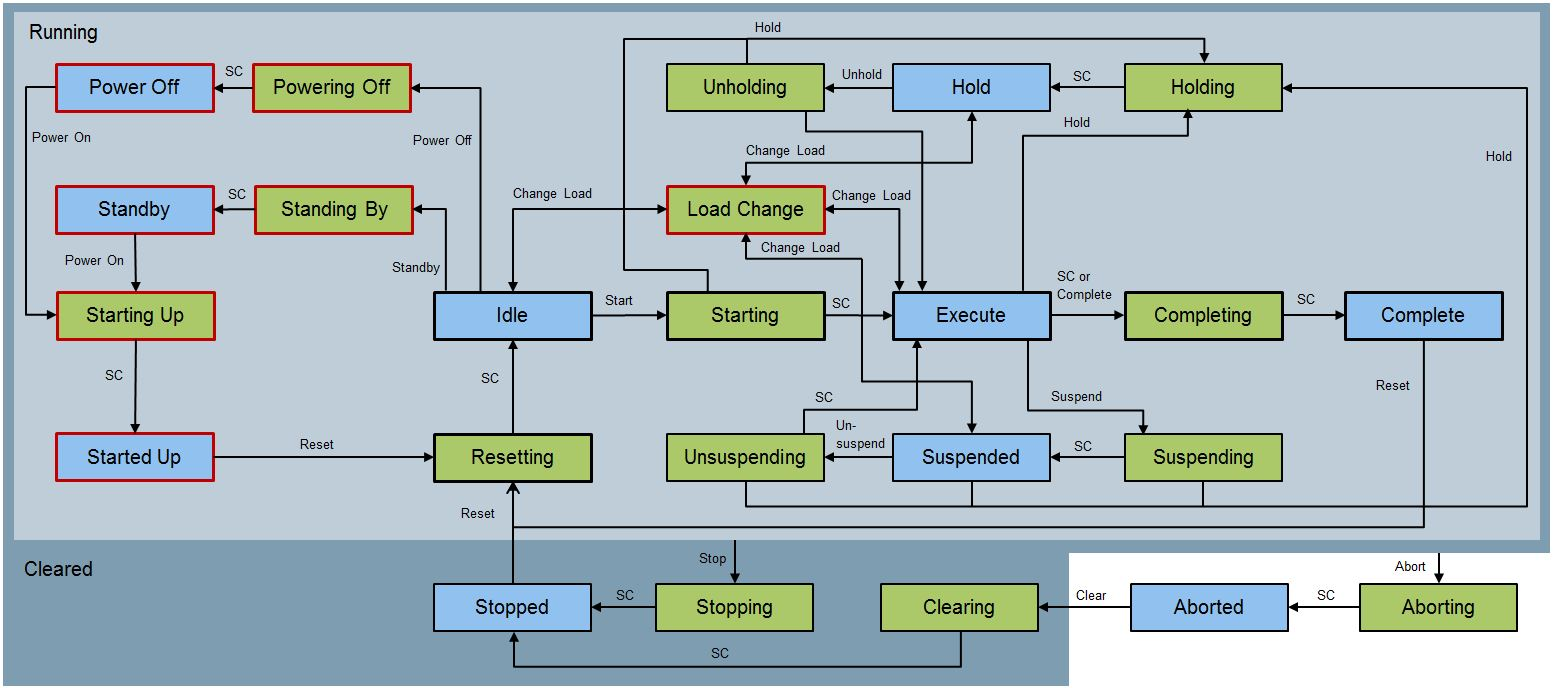
\includegraphics[scale=.40]{images/StateMachine_EFlex}
%
% If no graphics program available, insert a blank space i.e. use
%\picplace{5cm}{2cm} % Give the correct figure height and width in cm
%
\caption{Uniform state representation of a grid component. Every component can be stopped, halted, suspended, powered up or aborted. Once the component reach the $execute$-state then it begins to execute a production task, to generate energy or to store/release energy.}
\label{fig:state_chart}       % Give a unique label
\end{figure}



